\documentclass[11pt]{article}
\usepackage[margin=1in]{geometry}
\usepackage{booktabs,graphicx,amsmath,amssymb,microtype,xcolor,caption}
\usepackage[numbers,sort&compress]{natbib}
\usepackage{xurl}
\usepackage[hidelinks]{hyperref}
% generated by analysis/make_tables.py; do not edit
\newcommand{\accedgeBelNat}{0.409}
\newcommand{\accedgeMasNat}{0.243}
\newcommand{\accedgeMasRom}{0.044}
\newcommand{\accedgeSentNat}{0.472}
\newcommand{\accedgeSentRom}{0.366}
\newcommand{\accedgeSibNat}{0.475}
\newcommand{\accedgeSibRom}{0.235}
\newcommand{\accedgeXnliNat}{0.523}
\newcommand{\accedgeXnliRom}{0.445}
\newcommand{\accgemmaBelNat}{0.773}
\newcommand{\accgemmaMasNat}{0.689}
\newcommand{\accgemmaMasRom}{0.429}
\newcommand{\accgemmaSentNat}{0.590}
\newcommand{\accgemmaSentRom}{0.533}
\newcommand{\accgemmaSibNat}{0.853}
\newcommand{\accgemmaSibRom}{0.730}
\newcommand{\accgemmaXnliNat}{0.631}
\newcommand{\accgemmaXnliRom}{0.519}
\newcommand{\accjevBelNat}{0.918}
\newcommand{\accjevMasNat}{0.757}
\newcommand{\accjevMasRom}{0.481}
\newcommand{\accjevSentNat}{0.623}
\newcommand{\accjevSentRom}{0.527}
\newcommand{\accjevSibNat}{0.897}
\newcommand{\accjevSibRom}{0.725}
\newcommand{\accjevXnliNat}{0.751}
\newcommand{\accjevXnliRom}{0.572}
\newcommand{\accjuliaBelNat}{0.287}
\newcommand{\accjuliaSentNat}{0.403}
\newcommand{\accjuliaSentRom}{0.299}
\newcommand{\accjuliaSibNat}{0.520}
\newcommand{\accjuliaSibRom}{0.284}
\newcommand{\accjuliaXnliNat}{0.382}
\newcommand{\accjuliaXnliRom}{0.316}
\newcommand{\acckevmdBelNat}{0.561}
\newcommand{\acckevmdMasNat}{0.575}
\newcommand{\acckevmdMasRom}{0.226}
\newcommand{\acckevmdSentNat}{0.536}
\newcommand{\acckevmdSentRom}{0.408}
\newcommand{\acckevmdSibNat}{0.779}
\newcommand{\acckevmdSibRom}{0.451}
\newcommand{\acckevmdXnliNat}{0.624}
\newcommand{\acckevmdXnliRom}{0.475}
\newcommand{\acckevsmBelNat}{0.374}
\newcommand{\acckevsmMasNat}{0.372}
\newcommand{\acckevsmMasRom}{0.118}
\newcommand{\acckevsmSentNat}{0.359}
\newcommand{\acckevsmSentRom}{0.261}
\newcommand{\acckevsmSibNat}{0.632}
\newcommand{\acckevsmSibRom}{0.265}
\newcommand{\acckevsmXnliNat}{0.469}
\newcommand{\acckevsmXnliRom}{0.413}
\newcommand{\acclayabnBelNat}{0.313}
\newcommand{\acclayabnMasNat}{0.575}
\newcommand{\acclayabnMasRom}{0.077}
\newcommand{\acclayabnSentNat}{0.464}
\newcommand{\acclayabnSentRom}{0.216}
\newcommand{\acclayabnSibNat}{0.750}
\newcommand{\acclayabnSibRom}{0.250}
\newcommand{\acclayabnXnliNat}{0.625}
\newcommand{\acclayabnXnliRom}{0.435}
\newcommand{\acclayamlBelNat}{0.287}
\newcommand{\acclayamlMasNat}{0.179}
\newcommand{\acclayamlMasRom}{0.045}
\newcommand{\acclayamlSentNat}{0.263}
\newcommand{\acclayamlSentRom}{0.141}
\newcommand{\acclayamlSibNat}{0.588}
\newcommand{\acclayamlSibRom}{0.275}
\newcommand{\acclayamlXnliNat}{0.635}
\newcommand{\acclayamlXnliRom}{0.383}
\newcommand{\accliteBelNat}{0.577}
\newcommand{\accliteMasNat}{0.624}
\newcommand{\accliteMasRom}{0.121}
\newcommand{\accliteSentNat}{0.535}
\newcommand{\accliteSentRom}{0.343}
\newcommand{\accliteSibNat}{0.760}
\newcommand{\accliteSibRom}{0.265}
\newcommand{\accliteXnliNat}{0.704}
\newcommand{\accliteXnliRom}{0.463}
\newcommand{\accminiBelNat}{0.727}
\newcommand{\accminiMasNat}{0.749}
\newcommand{\accminiMasRom}{0.383}
\newcommand{\accminiSentNat}{0.579}
\newcommand{\accminiSentRom}{0.486}
\newcommand{\accminiSibNat}{0.838}
\newcommand{\accminiSibRom}{0.549}
\newcommand{\accminiXnliNat}{0.729}
\newcommand{\accminiXnliRom}{0.562}
\newcommand{\accnanoBelNat}{0.702}
\newcommand{\accnanoMasNat}{0.705}
\newcommand{\accnanoMasRom}{0.221}
\newcommand{\accnanoSentNat}{0.592}
\newcommand{\accnanoSentRom}{0.408}
\newcommand{\accnanoSibNat}{0.848}
\newcommand{\accnanoSibRom}{0.377}
\newcommand{\accnanoXnliNat}{0.746}
\newcommand{\accnanoXnliRom}{0.497}
\newcommand{\calCells}{32}
\newcommand{\calFull}{11}
\newcommand{\calOverAvg}{11}
\newcommand{\calUnderCells}{3}
\newcommand{\calUnderNames}{Kev-0.8B, Kev-4B and laya-bangla}
\newcommand{\consedge}{77}
\newcommand{\consgemma}{81}
\newcommand{\consjev}{93}
\newcommand{\consjulia}{35}
\newcommand{\conslayabn}{67}
\newcommand{\conslayaml}{53}
\newcommand{\conslite}{87}
\newcommand{\consnano}{89}
\newcommand{\dakBonfFail}{Julia-1}
\newcommand{\dakBonfNat}{11}
\newcommand{\dakBonfRule}{11}
\newcommand{\dakChance}{0.191}
\newcommand{\dakLeakJevNat}{0.695}
\newcommand{\dakN}{1{,}500}
\newcommand{\dakNTau}{11}
\newcommand{\dakNatBeatsRule}{7}
\newcommand{\dakNatDiffMax}{+4.5}
\newcommand{\dakNatDiffMin}{-1.8}
\newcommand{\dakNatLosesRule}{0}
\newcommand{\dakNatTied}{5}
\newcommand{\dakNsBeatsNat}{11}
\newcommand{\dakNsBeatsRule}{12}
\newcommand{\dakNsNatMax}{+8.9}
\newcommand{\dakNsNatMin}{+1.1}
\newcommand{\dakRuleDiffMax}{+12.9}
\newcommand{\dakRuleDiffMin}{+3.3}
\newcommand{\dakSystems}{12}
\newcommand{\dakTauNat}{0.85}
\newcommand{\dakTauRule}{0.89}
\newcommand{\dakedgeNat}{0.358}
\newcommand{\dakedgeNatVsRule}{+4.5}
\newcommand{\dakedgeNatVsRuleHi}{+6.5}
\newcommand{\dakedgeNatVsRuleLo}{+2.7}
\newcommand{\dakedgeNs}{0.442}
\newcommand{\dakedgeNsVsNat}{+8.4}
\newcommand{\dakedgeNsVsNatHi}{+10.9}
\newcommand{\dakedgeNsVsNatLo}{+6.0}
\newcommand{\dakedgeNsVsRule}{+12.9}
\newcommand{\dakedgeNsVsRuleHi}{+15.3}
\newcommand{\dakedgeNsVsRuleLo}{+10.5}
\newcommand{\dakedgeRule}{0.313}
\newcommand{\dakflashNat}{0.548}
\newcommand{\dakflashNatVsRule}{-1.0}
\newcommand{\dakflashNatVsRuleHi}{+2.2}
\newcommand{\dakflashNatVsRuleLo}{-4.2}
\newcommand{\dakflashNs}{0.632}
\newcommand{\dakflashNsVsNat}{+8.4}
\newcommand{\dakflashNsVsNatHi}{+12.6}
\newcommand{\dakflashNsVsNatLo}{+4.4}
\newcommand{\dakflashNsVsRule}{+7.4}
\newcommand{\dakflashNsVsRuleHi}{+11.4}
\newcommand{\dakflashNsVsRuleLo}{+3.0}
\newcommand{\dakflashRule}{0.558}
\newcommand{\dakgemmaNat}{0.670}
\newcommand{\dakgemmaNatVsRule}{+0.6}
\newcommand{\dakgemmaNatVsRuleHi}{+2.1}
\newcommand{\dakgemmaNatVsRuleLo}{-0.7}
\newcommand{\dakgemmaNs}{0.724}
\newcommand{\dakgemmaNsVsNat}{+5.4}
\newcommand{\dakgemmaNsVsNatHi}{+7.4}
\newcommand{\dakgemmaNsVsNatLo}{+3.3}
\newcommand{\dakgemmaNsVsRule}{+6.0}
\newcommand{\dakgemmaNsVsRuleHi}{+8.1}
\newcommand{\dakgemmaNsVsRuleLo}{+3.8}
\newcommand{\dakgemmaRule}{0.664}
\newcommand{\dakjevNat}{0.654}
\newcommand{\dakjevNatVsRule}{-1.8}
\newcommand{\dakjevNatVsRuleHi}{+0.1}
\newcommand{\dakjevNatVsRuleLo}{-3.7}
\newcommand{\dakjevNs}{0.733}
\newcommand{\dakjevNsVsNat}{+7.9}
\newcommand{\dakjevNsVsNatHi}{+10.1}
\newcommand{\dakjevNsVsNatLo}{+5.6}
\newcommand{\dakjevNsVsRule}{+6.1}
\newcommand{\dakjevNsVsRuleHi}{+8.5}
\newcommand{\dakjevNsVsRuleLo}{+3.9}
\newcommand{\dakjevRule}{0.672}
\newcommand{\dakjuliaNat}{0.461}
\newcommand{\dakjuliaNatVsRule}{+2.2}
\newcommand{\dakjuliaNatVsRuleHi}{+3.8}
\newcommand{\dakjuliaNatVsRuleLo}{+0.8}
\newcommand{\dakjuliaNs}{0.472}
\newcommand{\dakjuliaNsVsNat}{+1.1}
\newcommand{\dakjuliaNsVsNatHi}{+3.2}
\newcommand{\dakjuliaNsVsNatLo}{-1.1}
\newcommand{\dakjuliaNsVsRule}{+3.3}
\newcommand{\dakjuliaNsVsRuleHi}{+5.7}
\newcommand{\dakjuliaNsVsRuleLo}{+0.9}
\newcommand{\dakjuliaRule}{0.439}
\newcommand{\dakkevmdNat}{0.509}
\newcommand{\dakkevmdNatVsRule}{-0.1}
\newcommand{\dakkevmdNatVsRuleHi}{+1.8}
\newcommand{\dakkevmdNatVsRuleLo}{-1.9}
\newcommand{\dakkevmdNs}{0.597}
\newcommand{\dakkevmdNsVsNat}{+8.7}
\newcommand{\dakkevmdNsVsNatHi}{+11.1}
\newcommand{\dakkevmdNsVsNatLo}{+6.3}
\newcommand{\dakkevmdNsVsRule}{+8.7}
\newcommand{\dakkevmdNsVsRuleHi}{+10.9}
\newcommand{\dakkevmdNsVsRuleLo}{+6.3}
\newcommand{\dakkevmdRule}{0.510}
\newcommand{\dakkevsmNat}{0.329}
\newcommand{\dakkevsmNatVsRule}{+2.8}
\newcommand{\dakkevsmNatVsRuleHi}{+4.5}
\newcommand{\dakkevsmNatVsRuleLo}{+0.9}
\newcommand{\dakkevsmNs}{0.412}
\newcommand{\dakkevsmNsVsNat}{+8.3}
\newcommand{\dakkevsmNsVsNatHi}{+10.7}
\newcommand{\dakkevsmNsVsNatLo}{+5.7}
\newcommand{\dakkevsmNsVsRule}{+11.1}
\newcommand{\dakkevsmNsVsRuleHi}{+13.5}
\newcommand{\dakkevsmNsVsRuleLo}{+8.6}
\newcommand{\dakkevsmRule}{0.301}
\newcommand{\daklayabnNat}{0.261}
\newcommand{\daklayabnNatVsRule}{+3.0}
\newcommand{\daklayabnNatVsRuleHi}{+4.9}
\newcommand{\daklayabnNatVsRuleLo}{+1.2}
\newcommand{\daklayabnNs}{0.335}
\newcommand{\daklayabnNsVsNat}{+7.4}
\newcommand{\daklayabnNsVsNatHi}{+10.1}
\newcommand{\daklayabnNsVsNatLo}{+4.9}
\newcommand{\daklayabnNsVsRule}{+10.4}
\newcommand{\daklayabnNsVsRuleHi}{+13.0}
\newcommand{\daklayabnNsVsRuleLo}{+7.5}
\newcommand{\daklayabnRule}{0.231}
\newcommand{\daklayamlNat}{0.336}
\newcommand{\daklayamlNatVsRule}{+2.1}
\newcommand{\daklayamlNatVsRuleHi}{+4.0}
\newcommand{\daklayamlNatVsRuleLo}{+0.1}
\newcommand{\daklayamlNs}{0.373}
\newcommand{\daklayamlNsVsNat}{+3.7}
\newcommand{\daklayamlNsVsNatHi}{+6.3}
\newcommand{\daklayamlNsVsNatLo}{+0.9}
\newcommand{\daklayamlNsVsRule}{+5.8}
\newcommand{\daklayamlNsVsRuleHi}{+8.4}
\newcommand{\daklayamlNsVsRuleLo}{+3.3}
\newcommand{\daklayamlRule}{0.315}
\newcommand{\dakliteNat}{0.441}
\newcommand{\dakliteNatVsRule}{+2.3}
\newcommand{\dakliteNatVsRuleHi}{+4.1}
\newcommand{\dakliteNatVsRuleLo}{+0.5}
\newcommand{\dakliteNs}{0.481}
\newcommand{\dakliteNsVsNat}{+4.1}
\newcommand{\dakliteNsVsNatHi}{+6.5}
\newcommand{\dakliteNsVsNatLo}{+1.8}
\newcommand{\dakliteNsVsRule}{+6.4}
\newcommand{\dakliteNsVsRuleHi}{+8.9}
\newcommand{\dakliteNsVsRuleLo}{+4.0}
\newcommand{\dakliteRule}{0.417}
\newcommand{\dakminiNat}{0.543}
\newcommand{\dakminiNatVsRule}{+0.8}
\newcommand{\dakminiNatVsRuleHi}{+2.6}
\newcommand{\dakminiNatVsRuleLo}{-1.0}
\newcommand{\dakminiNs}{0.633}
\newcommand{\dakminiNsVsNat}{+8.9}
\newcommand{\dakminiNsVsNatHi}{+11.3}
\newcommand{\dakminiNsVsNatLo}{+6.6}
\newcommand{\dakminiNsVsRule}{+9.7}
\newcommand{\dakminiNsVsRuleHi}{+12.1}
\newcommand{\dakminiNsVsRuleLo}{+7.3}
\newcommand{\dakminiRule}{0.535}
\newcommand{\daknanoNat}{0.459}
\newcommand{\daknanoNatVsRule}{+1.9}
\newcommand{\daknanoNatVsRuleHi}{+4.0}
\newcommand{\daknanoNatVsRuleLo}{+0.1}
\newcommand{\daknanoNs}{0.534}
\newcommand{\daknanoNsVsNat}{+7.5}
\newcommand{\daknanoNsVsNatHi}{+9.9}
\newcommand{\daknanoNsVsNatLo}{+5.1}
\newcommand{\daknanoNsVsRule}{+9.4}
\newcommand{\daknanoNsVsRuleHi}{+12.0}
\newcommand{\daknanoNsVsRuleLo}{+6.9}
\newcommand{\daknanoRule}{0.440}
\newcommand{\dropMaxVal}{35.9}
\newcommand{\dropMinVal}{13.5}
\newcommand{\dropedge}{15.6}
\newcommand{\dropgemma}{13.8}
\newcommand{\dropjev}{18.1}
\newcommand{\dropjulia}{13.5}
\newcommand{\dropkevmd}{23.9}
\newcommand{\dropkevsm}{19.4}
\newcommand{\droplayabn}{35.9}
\newcommand{\droplayaml}{20.6}
\newcommand{\droplite}{35.8}
\newcommand{\dropmini}{22.9}
\newcommand{\dropnano}{34.7}
\newcommand{\eceedgeNatRaw}{0.174}
\newcommand{\eceedgeNatTs}{0.044}
\newcommand{\eceedgeRomRaw}{0.202}
\newcommand{\eceedgeRomTs}{0.085}
\newcommand{\ecegemmaNatRaw}{0.303}
\newcommand{\ecegemmaNatTs}{0.073}
\newcommand{\ecegemmaRomRaw}{0.391}
\newcommand{\ecegemmaRomTs}{0.082}
\newcommand{\ecejevNatRaw}{0.126}
\newcommand{\ecejevNatTs}{0.047}
\newcommand{\ecejevRomRaw}{0.146}
\newcommand{\ecejevRomTs}{0.095}
\newcommand{\ecejuliaNatRaw}{0.432}
\newcommand{\ecejuliaNatTs}{0.104}
\newcommand{\ecejuliaRomRaw}{0.494}
\newcommand{\ecejuliaRomTs}{0.154}
\newcommand{\ecelayabnNatRaw}{0.204}
\newcommand{\ecelayabnNatTs}{0.034}
\newcommand{\ecelayabnRomRaw}{0.331}
\newcommand{\ecelayabnRomTs}{0.172}
\newcommand{\ecelayamlNatRaw}{0.347}
\newcommand{\ecelayamlNatTs}{0.080}
\newcommand{\ecelayamlRomRaw}{0.530}
\newcommand{\ecelayamlRomTs}{0.209}
\newcommand{\eceliteNatRaw}{0.076}
\newcommand{\eceliteNatTs}{0.040}
\newcommand{\eceliteRomRaw}{0.172}
\newcommand{\eceliteRomTs}{0.108}
\newcommand{\eceminiNatRaw}{0.074}
\newcommand{\eceminiNatTs}{0.036}
\newcommand{\eceminiRomRaw}{0.079}
\newcommand{\eceminiRomTs}{0.035}
\newcommand{\ecenanoNatRaw}{0.083}
\newcommand{\ecenanoNatTs}{0.041}
\newcommand{\ecenanoRomRaw}{0.122}
\newcommand{\ecenanoRomTs}{0.054}
\newcommand{\flashNmax}{405}
\newcommand{\flashNmin}{204}
\newcommand{\gateTarget}{90}
\newcommand{\gatejevNatAcc}{91}
\newcommand{\gatejevNatCov}{69}
\newcommand{\gatejevNatN}{1{,}036}
\newcommand{\gatejevRomAcc}{88}
\newcommand{\gatejevRomCov}{23}
\newcommand{\gatejevRomN}{341}
\newcommand{\gatelayabnNatAcc}{91}
\newcommand{\gatelayabnNatCov}{32}
\newcommand{\gatelayabnNatN}{475}
\newcommand{\gatelayabnRomAcc}{17}
\newcommand{\gatelayabnRomCov}{1}
\newcommand{\gatelayabnRomN}{12}
\newcommand{\gateliteNatAcc}{90}
\newcommand{\gateliteNatCov}{43}
\newcommand{\gateliteRomAcc}{47}
\newcommand{\gateliteRomCov}{7}
\newcommand{\gateminiNatAcc}{90}
\newcommand{\gateminiNatCov}{68}
\newcommand{\gateminiNatN}{1{,}020}
\newcommand{\gateminiRomAcc}{83}
\newcommand{\gateminiRomCov}{22}
\newcommand{\gateminiRomN}{335}
\newcommand{\gpuHours}{30}
\newcommand{\jevBelebele}{0.918}
\newcommand{\jevBelebeleHi}{0.936}
\newcommand{\jevBelebeleLo}{0.897}
\newcommand{\jevBelebeleZenodo}{0.9167}
\newcommand{\jevRequests}{99{,}828}
\newcommand{\jevRetestSame}{99}
\newcommand{\jevTokensM}{53.6}
\newcommand{\jevUsd}{2.25}
\newcommand{\juliaXnliEceRaw}{0.420}
\newcommand{\juliaXnliEceTs}{0.098}
\newcommand{\labelMaxDiff}{0.8}
\newcommand{\layabnNativeMassive}{0.575}
\newcommand{\layabnNativeSentnob}{0.464}
\newcommand{\layabnNativeSib}{0.750}
\newcommand{\layabnNativeXnli}{0.625}
\newcommand{\layamlNativeMassive}{0.179}
\newcommand{\layamlNativeSentnob}{0.263}
\newcommand{\layamlNativeSib}{0.588}
\newcommand{\layamlNativeXnli}{0.635}
\newcommand{\layamlSentBn}{0.376}
\newcommand{\layamlSentDefault}{0.263}
\newcommand{\layamlSentOpts}{0.321}
\newcommand{\lookupKept}{34{,}870}
\newcommand{\lookupRemoved}{4{,}144}
\newcommand{\nbelebele}{900}
\newcommand{\nbnli}{4895}
\newcommand{\nmassive}{2974}
\newcommand{\nsentnob}{1586}
\newcommand{\nsib}{204}
\newcommand{\pdBel}{-14.4}
\newcommand{\pdBelHi}{-11.9}
\newcommand{\pdBelLo}{-16.8}
\newcommand{\pdFlashBel}{-7.0}
\newcommand{\pdFlashBelHi}{-3.4}
\newcommand{\pdFlashBelLo}{-10.9}
\newcommand{\pdFlashMas}{+2.0}
\newcommand{\pdFlashMasHi}{+5.0}
\newcommand{\pdFlashMasLo}{-1.5}
\newcommand{\pdFlashSent}{-2.0}
\newcommand{\pdFlashSentHi}{+2.0}
\newcommand{\pdFlashSentLo}{-6.2}
\newcommand{\pdFlashSib}{-0.5}
\newcommand{\pdFlashSibHi}{+3.9}
\newcommand{\pdFlashSibLo}{-4.9}
\newcommand{\pdFlashXnli}{+7.5}
\newcommand{\pdFlashXnliHi}{+11.9}
\newcommand{\pdFlashXnliLo}{+3.3}
\newcommand{\pdMas}{-0.8}
\newcommand{\pdMasHi}{+1.4}
\newcommand{\pdMasLo}{-3.0}
\newcommand{\pdSent}{-2.0}
\newcommand{\pdSentHi}{-0.4}
\newcommand{\pdSentLo}{-3.5}
\newcommand{\pdSib}{-4.4}
\newcommand{\pdSibHi}{+0.0}
\newcommand{\pdSibLo}{-8.6}
\newcommand{\pdXnli}{-0.5}
\newcommand{\pdXnliHi}{+1.9}
\newcommand{\pdXnliLo}{-2.6}
\newcommand{\sentMajorityFone}{0.195}
\newcommand{\sentUniformFone}{0.328}
\newcommand{\subflashXnli}{0.828}
\newcommand{\subjevXnli}{0.752}
\newcommand{\tsCells}{26}
\newcommand{\tsLowered}{26}
\newcommand{\tsSystems}{9}

\newcommand{\TK}[1]{\textcolor{red}{[TK: #1]}}
\captionsetup{font=small,labelfont=bf}
\renewcommand{\arraystretch}{1.05}
\emergencystretch=3em

\title{Decision Models on Bengali:\\Accuracy, Calibration and Robustness to Romanization}
\author{Ismail Hossain Polas\\Jahangirnagar University\\\texttt{ismailhossainpolash@gmail.com}}
\date{\today}

\begin{document}
\maketitle

\begin{abstract}
\noindent Decision models answer a typed question in one forward pass and return a probability for every option.
I tested one hosted decision model, Jev, ten open decision models and one general-purpose language model on five Bengali tasks, zero-shot.
Jev scored highest on all five tasks among the models run on the full test sets; on Belebele it reached \jevBelebele{} (95\% CI \jevBelebeleLo{} to \jevBelebeleHi).
Rule-based romanization lowered every system's accuracy on every task it was applied to, by \dropMinVal{} to \dropMaxVal{} points on average.
To ask whether such tool-made romanization overstates the penalty, I compared it with the Latin-script spelling that native speakers wrote for \dakN{} Bengali Wikipedia sentences (the Dakshina dataset).
On these sentences all \dakSystems{} systems kept their own Bengali-script topic answer more often under the native-speaker romanization than under the rule-based one, by \dakRuleDiffMin{} to \dakRuleDiffMax{} points, and every interval excludes zero.
Jev kept it \dakjevNs{} of the time against \dakjevRule{}.
A romanizer tuned on typed Banglish changed little: it differed from the rule-based one by \dakNatDiffMin{} to \dakNatDiffMax{} points. The ordering of systems was almost the same under both spellings (Kendall $\tau=\dakTauRule$).
Every open model was overconfident on Bengali text, and one temperature fitted on a separate development set removed most of that, but less of it on rule-based romanized text.
Code, tables and per-sentence predictions are at \url{https://github.com/ihpolash/system-one-testing-for-bengali}.
\end{abstract}

\section{Introduction}
A decision model reads a text and a typed question and returns one probability per option, without generating anything.
That makes the output easy to act on: a pipeline can accept confident answers and send the rest to a larger model or a person \citep{deusser2026jev,nandakishore2026laya}.
Nearly all of the evidence for this comes from English.
The one study that left English shows why that matters. On Chinese tasks Laya-multilingual scored 40.2\% where Jev scored 68.4\% \citep{wang2026chinesejev}.
For Bengali I found only the per-language Belebele and SIB-200 numbers that ship with the Jev benchmark \citep{deusser2026jev}. I found no study that asked whether a decision model's confidence still means something in Bengali.

Bengali has a second difficulty. A great deal of everyday Bengali is typed in Latin letters, with no standard spelling.
Work on other Indic languages and on Bangla dialects tests romanized text produced by a transliteration tool, and finds large losses \citep{khullar2025scriptgap,jawad2026fivedialects}.
A tool applies one rule per letter. People do not.
I found no measurement, for Bengali, of how far the loss on tool-made romanization differs from the loss on what native speakers actually write.

The Dakshina dataset makes that measurement possible: 10,000 Bengali Wikipedia sentences that native speakers romanized by hand \citep{roark2020dakshina}.
It has no task labels, so I measure something else: how often a system's answer to a topic question survives the change of script (Section~\ref{sec:dak}).
Around it sits a zero-shot benchmark of twelve systems on five tasks, with calibration, risk--coverage and option-order analyses (Section~\ref{sec:results}).
Every number here is produced by the released code, and the harness reproduces published numbers from independent groups for Jev, Laya-multilingual and laya-bangla (Section~\ref{sec:audit}).
This is not the first Bengali result for any decision model, since Jev's Belebele and SIB-200 numbers exist. Kev-9B, Kev-27B, d3-27B and Microsoft-Decision-1 are not covered.

\section{Related work}
\label{sec:related}
Table~\ref{tab:gap} shows what the closest studies cover.
In English, decision models have been checked for calibration \citep{nandakishore2026laya}, for annotation work with open models \citep{ibrahim2026annotation}, for sensitivity to option names \citep{sun2026typesafe} and to option order \citep{li2026readout}, and for cost and wording robustness \citep{sharma2026typedbench}.
Other languages are thin. Chinese-Jev trains a Chinese model \citep{wang2026chinesejev}, and one paper compares Jev's cultural-value answers in English and Arabic \citep{asseri2026calibrated}.
Script robustness has been studied for generative models only \citep{khullar2025scriptgap,jawad2026fivedialects}, and the Bengali half of the large romanization corpus of \citet{gharami2025romanized} is generated by rule, not typed by people.
For calibration and selective prediction I use the standard measures \citep{guo2017calibration,geifman2017selective}; the option-rotation test follows \citet{zheng2024selectors}.
The tasks are Belebele \citep{bandarkar2023belebele}, SIB-200 \citep{adelani2023sib200}, MASSIVE \citep{fitzgerald2022massive}, SentNoB \citep{islam2021sentnob} and the Bengali translation of XNLI; the romanization data are from Dakshina \citep{roark2020dakshina}.
\begin{table}[t]
\centering\footnotesize
\resizebox{\linewidth}{!}{\begin{tabular}{@{}lccccc@{}}\toprule
Study & Decision models & Bengali & Romanized & Calibration & Human-typed text \\\midrule
\citet{deusser2026jev} & Jev only & per-language file & Belebele, SIB-200 & yes & no \\
\citet{wang2026chinesejev} & trained model & no & no & yes & no \\
\citet{khullar2025scriptgap} & no & no & tool-made & routing only & no \\
\citet{jawad2026fivedialects} & no & dialects & tool-made & no & no \\
This paper & 12 systems & 5 tasks & rule-based, natural-style, native-speaker & yes & yes (\dakN{} sentences) \\
\bottomrule\end{tabular}}
\caption{What each closest study covers, from reading the papers. A ``no'' means the paper does not report it.}
\label{tab:gap}
\end{table}

\section{Benchmark}
\label{sec:method}
\paragraph{Models.}
Jev (\texttt{jev-1.13.0}) is reached through its API.
The open models ran on Kaggle GPUs: Laya-multilingual, an mmBERT-based encoder \citep{marone2025mmbert}; laya-bangla v2, a Bangla fine-tune of it (commit \texttt{4c5eb48932}); Julia-1, with 144M parameters; the vLLM-SR Decision 3.0 models d3-edge, d3-lite, d3-nano, d3-mini and d3-flash \citep{liu2026vllmsr}; and Kev-0.8B and Kev-4B (release 1.0, tag \texttt{v1.0}), served with the project's own code in bf16 with its shipped temperature.
Kev's model cards list English as its only language and name other languages as a known weakness.
Kev-4B sits at the memory limit of a 15 GB T4, so for it I switched off CUDA-graph replay and the prefix cache, which change speed and memory but not the model, after a first run ran out of memory.
Kev was scored on the test sets and on the Dakshina sentences only, so it is missing from the calibration and option-order results.
d3-flash has 9B parameters and did not fit comfortably, so it ran 4-bit (NF4), on a hash-ordered subset of about \flashNmax{} items per task and of 500 Dakshina sentences.
Gemma-4-E4B-it is not a decision model; it serves as a baseline, with each option scored by the next-token probability of its label and the probabilities normalized over the options.
Kev-9B and Kev-27B do not fit on that GPU, and d3-27B and Microsoft-Decision-1 (API only) were not run. Exact identifiers and settings are in \texttt{docs/MODELS.md}.

\paragraph{Tasks.}
The five tasks are in Table~\ref{tab:tasks}.
Each item is a single-choice question with English instructions and option names; only the passage or utterance changes between conditions. The exact question structure for every task is in \texttt{docs/PROMPTS.md} in the repository.
I cut XNLI-bn and MASSIVE to hash-ordered subsets of 1,500 items so that any smaller run is nested in a larger one.
Bengali option names changed Jev's accuracy by at most \labelMaxDiff{} points on SentNoB, XNLI-bn and SIB-200, so I kept English names throughout.
The metric is accuracy, and macro-F1 for SentNoB.
\begin{table}[t]
\centering\footnotesize
\resizebox{\linewidth}{!}{\begin{tabular}{@{}llllll@{}}\toprule
Dataset & Task & Options & Metric & Text origin & Test items (all / used) \\\midrule
Belebele & reading comprehension & 4 options & accuracy & human translation (FLORES-200) & 900 / 900 \\
SIB-200 & topic & 7 options & accuracy & human translation (FLORES-200) & 204 / 204 \\
XNLI-bn & natural language inference & 3 options & accuracy & machine translation of XNLI & 4,895 / 1,500 \\
MASSIVE bn-BD & intent & 60 options & accuracy & human translation & 2,974 / 1,500 \\
SentNoB & sentiment & 3 options & macro-F1 & native social-media comments & 1,586 / 1,586 \\
\bottomrule\end{tabular}
}
\caption{Tasks. XNLI-bn is the machine-translated Bengali XNLI, so its text is translationese; SentNoB is the only native Bengali set. MASSIVE is posed with all 60 intents; the test items use 59 of them. The SentNoB split is a third-party mirror whose provenance I could not verify.}
\label{tab:tasks}
\end{table}

\paragraph{Romanization.}
\emph{Rule-based romanization} maps each letter to Latin letters by a fixed rule set, without diacritics. It is applied to the test sets of four tasks (Belebele passages were not romanized).
\emph{Natural-style romanization} replaces each word with its most frequent spelling in a public corpus of typed Banglish (nahidstaq/bangla-transliteration-data) and falls back to rules tuned on held-out words from that corpus.
That corpus turned out to contain \lookupRemoved{} Dakshina sentences with their native-speaker romanization, so my first version had effectively seen the target spellings and scored \dakLeakJevNat{} for Jev. I removed every pair that matches a Dakshina string, rebuilt the lookup from the remaining \lookupKept{} sentences, re-checked the rule settings and reran; all natural-style numbers here use the rebuilt version.
\emph{Native-speaker romanization} is the Latin-script text in Dakshina, which native speakers wrote for each Bengali sentence without a transliteration tool; a second set of annotators transcribed it back to Bengali script to validate it \citep{roark2020dakshina}.

\paragraph{Dakshina sentences.}
I kept the sentences of 6 to 40 words whose romanization has no Bengali script and dropped duplicates, which left 8,244 of the 10,000, and used the first \dakN{} in hash order (500 for d3-flash, nested in them).
There are no task labels. Every system answers one seven-way topic question about each sentence, with the SIB-200 topics, in four spellings: Bengali script, native-speaker, rule-based and natural-style romanization.
The measure is agreement: the share of sentences whose top option is unchanged from the system's own answer on the Bengali-script sentence. I also report the mean total-variation distance between the two probability vectors, and the agreement expected by chance, $\sum_c p_{\text{Bengali}}(c)\,p_{\text{romanized}}(c)$ (\dakChance{} on average).
Agreement is not accuracy: a system that is wrong on the Bengali sentence can agree with itself on the romanization.

\paragraph{Statistics.}
Intervals are 95\% percentile bootstraps (seed 0). On the test sets they resample premise or passage clusters (Belebele, XNLI-bn) or items, 1,000 times (400 for the SentNoB macro-F1, 500 for paired differences). On the Dakshina sentences they resample sentences 1,000 times, and every comparison between spellings is a paired difference on the same sentences.
Calibration is measured with expected calibration error over 15 equal-width bins (ECE), the signed gap between confidence and accuracy, the Brier score and risk--coverage curves. ECE is computed within each task on the full test sets and then averaged without weights over XNLI-bn, MASSIVE and SentNoB (Table~\ref{tab:cal}; per task in Table~\ref{tab:caltasks}), because the tasks differ in the number of options and in label balance.
Temperature scaling uses one scalar per model and task. It minimizes the mean negative log-likelihood over a grid of 41 log-spaced temperatures from 0.2 to 6, on a development split of 1,500 items (XNLI-bn, MASSIVE, SentNoB) that is disjoint from the test items and holds Bengali text only. The fitted temperature is then applied unchanged to the test items in Bengali and in rule-based romanization; no test label enters the fit. Belebele and SIB-200 have no development split, and d3-flash and Kev were not run on one, so they have no scaled results. The confidence gate uses the same development split: its threshold is the smallest one whose accepted dev accuracy reaches \gateTarget\%, with at least 5\% coverage.
Option-order sensitivity uses three cyclic rotations of the options.
I report no significance tests. The main comparison is native-speaker against rule-based romanization on the Dakshina sentences; every other comparison is descriptive, and none is corrected for the number of comparisons.

\section{Results}
\label{sec:results}
\subsection{Accuracy on Bengali script and rule-based romanization}
Table~\ref{tab:main} and Figure~\ref{fig:script} give the main results. Every system is less accurate on rule-based romanization than on Bengali script on every task where both were run: by \dropMinVal{} to \dropMaxVal{} points on average over the tasks, \dropjev{} for Jev.
Jev has the highest point estimate on every task among the models run on the full sets.
The closest open model is d3-nano on XNLI-bn (\accnanoXnliNat{} against \accjevXnliNat), with d3-mini at \accminiXnliNat, and the intervals in Table~\ref{tab:ci} overlap.
d3-flash, on its subset, scores \subflashXnli{} on XNLI-bn against Jev's \subjevXnli{}, and trails on Belebele (Table~\ref{tab:flash}). It is above Jev on three tasks, but with \flashNmin{} to \flashNmax{} items per task I read that as level.
Kev-4B lands next to d3-lite: \acckevmdBelNat{} on Belebele against \accliteBelNat, \acckevmdSibNat{} on SIB-200 against \accliteSibNat, \acckevmdSentNat{} on SentNoB against \accliteSentNat, and below it on XNLI-bn (\acckevmdXnliNat{} against \accliteXnliNat) and MASSIVE (\acckevmdMasNat{} against \accliteMasNat). Kev-0.8B scores \acckevsmSibNat{} on SIB-200 and \acckevsmMasNat{} on MASSIVE, and falls in the lower group with d3-edge and Laya-multilingual. Both Kev models are well below Jev on every task.
Gemma-4-E4B holds up best under rule-based romanization: on SIB-200 it keeps \accgemmaSibRom{} of \accgemmaSibNat, where d3-mini keeps \accminiSibRom{} of \accminiSibNat.
laya-bangla beats its base model on SIB-200 (\acclayabnSibNat{} against \acclayamlSibNat) and on MASSIVE (\acclayabnMasNat{} against \acclayamlMasNat) and still sits below Jev, d3-mini and Gemma-4-E4B on every task.
On SentNoB, always answering with the majority class scores a macro-F1 of \sentMajorityFone{} and uniform random guessing \sentUniformFone{}. Laya-multilingual reaches only \acclayamlSentNat, below random guessing, Kev-0.8B \acckevsmSentNat{} and Julia-1 \accjuliaSentNat. Julia-1 cannot take the 60-option MASSIVE menu at all.
Laya-multilingual's SentNoB score also depends on the wording of the question: macro-F1 is \layamlSentDefault{} with my default instruction, \layamlSentOpts{} with option names only, and \layamlSentBn{} with Bengali wording. I report the default and flag the range.
\begin{table}[t]
\centering\footnotesize
\begin{tabular}{@{}lccccc@{}}\toprule
Model & Belebele & SIB-200 & XNLI-bn & MASSIVE & SentNoB \\\midrule
Jev & 0.918 & 0.897 (0.725) & 0.751 (0.572) & 0.757 (0.481) & 0.623 (0.527) \\
Gemma-4-E4B & 0.773 & 0.853 (0.730) & 0.631 (0.519) & 0.689 (0.429) & 0.590 (0.533) \\
d3-mini & 0.727 & 0.838 (0.549) & 0.729 (0.562) & 0.749 (0.383) & 0.579 (0.486) \\
d3-nano & 0.702 & 0.848 (0.377) & 0.746 (0.497) & 0.705 (0.221) & 0.592 (0.408) \\
Kev-4B & 0.561 & 0.779 (0.451) & 0.624 (0.475) & 0.575 (0.226) & 0.536 (0.408) \\
d3-lite & 0.577 & 0.760 (0.265) & 0.704 (0.463) & 0.624 (0.121) & 0.535 (0.343) \\
laya-bangla & 0.313 & 0.750 (0.250) & 0.625 (0.435) & 0.575 (0.077) & 0.464 (0.216) \\
d3-edge & 0.409 & 0.475 (0.235) & 0.523 (0.445) & 0.243 (0.044) & 0.472 (0.366) \\
Kev-0.8B & 0.374 & 0.632 (0.265) & 0.469 (0.413) & 0.372 (0.118) & 0.359 (0.261) \\
Laya-multilingual & 0.287 & 0.588 (0.275) & 0.635 (0.383) & 0.179 (0.045) & 0.263 (0.141) \\
Julia-1 & 0.287 & 0.520 (0.284) & 0.382 (0.316) & -- & 0.403 (0.299) \\
\midrule
Majority class & -- & 0.250 & 0.342 & 0.071 & 0.195 \\
Uniform random & 0.250 & 0.143 & 0.333 & 0.017 & 0.328 \\
\bottomrule\end{tabular}

\caption{Accuracy on Bengali script, and in brackets on rule-based romanization, rotation 0 (SentNoB: macro-F1). Belebele passages were not romanized. Julia-1 cannot take the 60 options of MASSIVE. Majority class: the share of the most frequent label in the test items (for SentNoB, the macro-F1 of always predicting it); Belebele's answer positions rotate, so it has none. Uniform random: one over the number of options (for SentNoB, the expected macro-F1 of random guessing). Intervals are in Table~\ref{tab:ci}.}
\label{tab:main}
\end{table}
\begin{table}[t]
\centering\footnotesize
\begin{tabular}{@{}lccccc@{}}\toprule
On the d3-flash subset & Belebele & SIB-200 & XNLI-bn & MASSIVE & SentNoB \\\midrule
Jev & 0.840 & 0.897 (0.725) & 0.752 (0.557) & 0.799 (0.519) & 0.637 (0.577) \\
d3-flash (4-bit) & 0.730 & 0.892 (0.627) & 0.828 (0.598) & 0.819 (0.412) & 0.653 (0.519) \\
\bottomrule\end{tabular}

\caption{d3-flash (4-bit) and Jev on the same hash-ordered subset (\flashNmin{} to \flashNmax{} items per task); romanized in brackets. d3-flash is the 9B checkpoint in 4-bit quantization.}
\label{tab:flash}
\end{table}
\begin{figure}[t]
\centering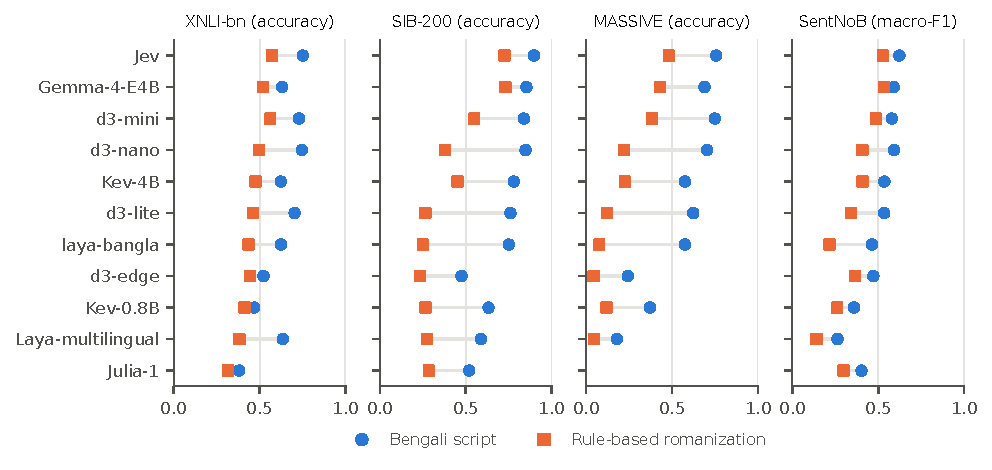
\includegraphics[width=\linewidth]{figures/fig2_script_gap}
\caption{Bengali script against rule-based romanization for each model and task. Lines join the two conditions for the same model.}
\label{fig:script}
\end{figure}


\subsection{Romanization written by native speakers}
\label{sec:dak}
Table~\ref{tab:dak} and Figure~\ref{fig:dak} give the agreement for all twelve systems.
Under native-speaker romanization every system kept its Bengali-script answer more often than under rule-based romanization, by \dakRuleDiffMin{} to \dakRuleDiffMax{} points, and the interval excludes zero for all \dakNsBeatsRule{}. For Jev the gain is \dakjevNsVsRule{} points (95\% CI \dakjevNsVsRuleLo{} to \dakjevNsVsRuleHi): it kept its answer on \dakjevNs{} of the sentences against \dakjevRule{}, where chance is about \dakChance{}.
The smallest gain is Julia-1's, at \dakjuliaNsVsRule{} points, which fits a system that sits near its floor; the largest is d3-edge's, at \dakedgeNsVsRule{}.
Natural-style romanization, which looks each word up in a corpus of typed Banglish, ends up close to the rule-based text. It differs from the rule-based spelling by \dakNatDiffMin{} to \dakNatDiffMax{} points: it keeps the Bengali answer more often for \dakNatBeatsRule{} systems, makes no detectable difference for \dakNatTied{}, and is worse for \dakNatLosesRule{}. For Jev the difference is \dakjevNatVsRule{} points (\dakjevNatVsRuleLo{} to \dakjevNatVsRuleHi). Native-speaker romanization beats it for \dakNsBeatsNat{} of the \dakSystems{} systems, by \dakNsNatMin{} to \dakNsNatMax{} points, and the remaining system is within noise.
Tuning a romanizer on typed Banglish therefore gives little, and the gap to what native speakers write remains.
The probability vectors tell the same story: the total-variation distance from the Bengali answer is smaller under native-speaker romanization for every system (Table~\ref{tab:daktv}).

The ordering of systems moves little. Over the \dakNTau{} systems with all \dakN{} sentences, Kendall $\tau$ between the ordering under native-speaker romanization and under rule-based romanization is \dakTauRule.
Rule-based romanization therefore ranks systems in nearly the same order as real typing, and overstates how far their answers move.
Two limits matter. These are Wikipedia sentences and one topic question, not the five tasks, and the measure is consistency with the system's own Bengali answer, not correctness.
\begin{figure}[t]
\centering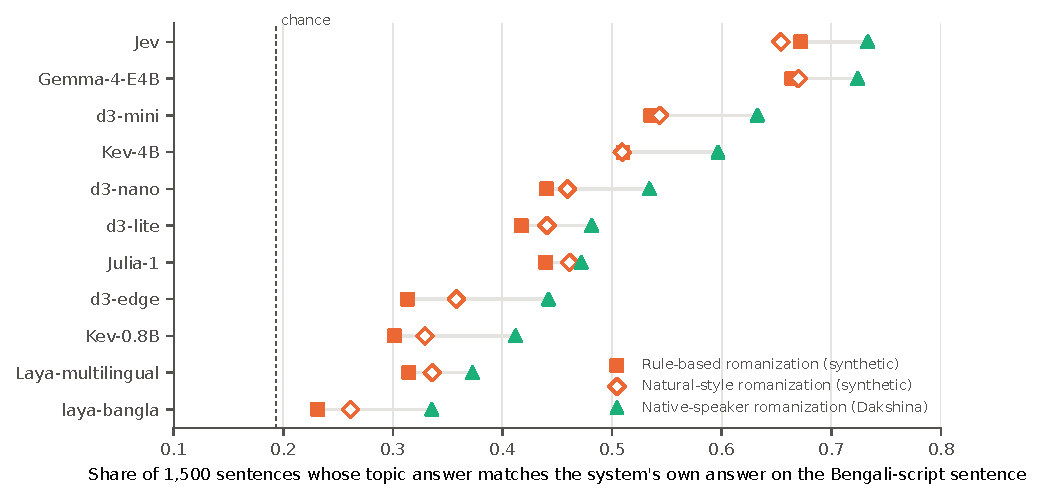
\includegraphics[width=.92\linewidth]{figures/fig1_dakshina}
\caption{Share of \dakN{} Dakshina sentences whose topic answer matches the system's own answer on the Bengali-script sentence, for three spellings of the same sentence. Chance is the dashed line. Intervals are in Table~\ref{tab:dak}; d3-flash (500 sentences) is omitted here.}
\label{fig:dak}
\end{figure}
\begin{table}[t]
\centering\footnotesize
\resizebox{\linewidth}{!}{\begin{tabular}{@{}lrccccc@{}}\toprule
 & & \multicolumn{3}{c}{Agreement with own Bengali answer} & \multicolumn{2}{c}{Difference in points (95\% CI)} \\\cmidrule(lr){3-5}\cmidrule(l){6-7}
Model & Sentences & Native-speaker & Natural-style & Rule-based & Native-speaker $-$ rule-based & Native-speaker $-$ natural-style \\\midrule
Jev & 1,500 & 0.733 & 0.654 & 0.672 & +6.1 [+3.9, +8.5] & +7.9 [+5.6, +10.1] \\
d3-flash (4-bit)$^\dagger$ & 500 & 0.632 & 0.548 & 0.558 & +7.4 [+3.0, +11.4] & +8.4 [+4.4, +12.6] \\
Gemma-4-E4B & 1,500 & 0.724 & 0.670 & 0.664 & +6.0 [+3.8, +8.1] & +5.4 [+3.3, +7.4] \\
d3-mini & 1,500 & 0.633 & 0.543 & 0.535 & +9.7 [+7.3, +12.1] & +8.9 [+6.6, +11.3] \\
d3-nano & 1,500 & 0.534 & 0.459 & 0.440 & +9.4 [+6.9, +12.0] & +7.5 [+5.1, +9.9] \\
Kev-4B & 1,500 & 0.597 & 0.509 & 0.510 & +8.7 [+6.3, +10.9] & +8.7 [+6.3, +11.1] \\
d3-lite & 1,500 & 0.481 & 0.441 & 0.417 & +6.4 [+4.0, +8.9] & +4.1 [+1.8, +6.5] \\
laya-bangla & 1,500 & 0.335 & 0.261 & 0.231 & +10.4 [+7.5, +13.0] & +7.4 [+4.9, +10.1] \\
d3-edge & 1,500 & 0.442 & 0.358 & 0.313 & +12.9 [+10.5, +15.3] & +8.4 [+6.0, +10.9] \\
Kev-0.8B & 1,500 & 0.412 & 0.329 & 0.301 & +11.1 [+8.6, +13.5] & +8.3 [+5.7, +10.7] \\
Laya-multilingual & 1,500 & 0.373 & 0.336 & 0.315 & +5.8 [+3.3, +8.4] & +3.7 [+0.9, +6.3] \\
Julia-1 & 1,500 & 0.472 & 0.461 & 0.439 & +3.3 [+0.9, +5.7] & +1.1 [-1.1, +3.2] \\
\bottomrule\end{tabular}
}
\caption{Agreement with the system's own Bengali-script answer on Dakshina sentences, and paired differences in points with 95\% bootstrap intervals. $^\dagger$d3-flash is 4-bit and covers a 500-sentence subset.}
\label{tab:dak}
\end{table}

\subsection{Calibration and selective prediction}
Overconfidence differs a lot between models. Raw ECE on Bengali script, averaged over the three tasks as described above, runs from \eceminiNatRaw{} for d3-mini to \ecejuliaNatRaw{} for Julia-1 (Table~\ref{tab:cal}).
One temperature, fitted on a separate Bengali development split, lowers ECE for every model on Bengali text; for Julia-1 on XNLI-bn it takes ECE from \juliaXnliEceRaw{} to \juliaXnliEceTs.
On rule-based romanized text the same temperature leaves a higher ECE for eight of the nine models with a development run (Kev and d3-flash have none). d3-mini is the exception. Jev's scaled ECE is \ecejevRomTs{} on romanized text against \ecejevNatTs{} on Bengali, and laya-bangla's is \ecelayabnRomTs{} against \ecelayabnNatTs.
Figure~\ref{fig:rel} shows the reliability curves and Figure~\ref{fig:rc} the risk--coverage curves. Confidence still ranks answers within each condition, but rule-based romanization lowers accuracy at every coverage level, including among the most confident answers.
\begin{table}[t]
\centering\footnotesize
\begin{tabular}{@{}lcccc@{}}\toprule
 & \multicolumn{2}{c}{Bengali script} & \multicolumn{2}{c}{Rule-based romanization} \\\cmidrule(lr){2-3}\cmidrule(l){4-5}
Model & ECE raw & ECE scaled & ECE raw & ECE scaled \\\midrule
Jev & 0.126 & 0.047 & 0.146 & 0.095 \\
Gemma-4-E4B & 0.303 & 0.073 & 0.391 & 0.082 \\
d3-mini & 0.074 & 0.036 & 0.079 & 0.035 \\
d3-nano & 0.083 & 0.041 & 0.122 & 0.054 \\
d3-lite & 0.076 & 0.040 & 0.172 & 0.108 \\
d3-edge & 0.174 & 0.044 & 0.202 & 0.085 \\
laya-bangla & 0.204 & 0.034 & 0.331 & 0.172 \\
Laya-multilingual & 0.347 & 0.080 & 0.530 & 0.209 \\
Julia-1 & 0.432 & 0.104 & 0.494 & 0.154 \\
\bottomrule\end{tabular}

\caption{ECE (15 bins) on Bengali script and rule-based romanization, before and after one temperature fitted on a native-text development split. Mean over XNLI-bn, MASSIVE and SentNoB.}
\label{tab:cal}
\end{table}
\begin{figure}[t]
\centering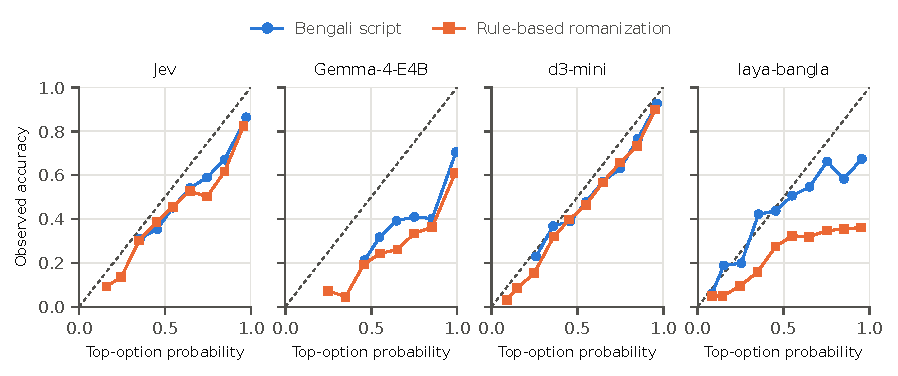
\includegraphics[width=\linewidth]{figures/fig3_reliability}
\caption{Reliability of four models on MASSIVE, XNLI-bn and SentNoB pooled. The dashed line is perfect calibration.}
\label{fig:rel}
\end{figure}
\begin{figure}[t]
\centering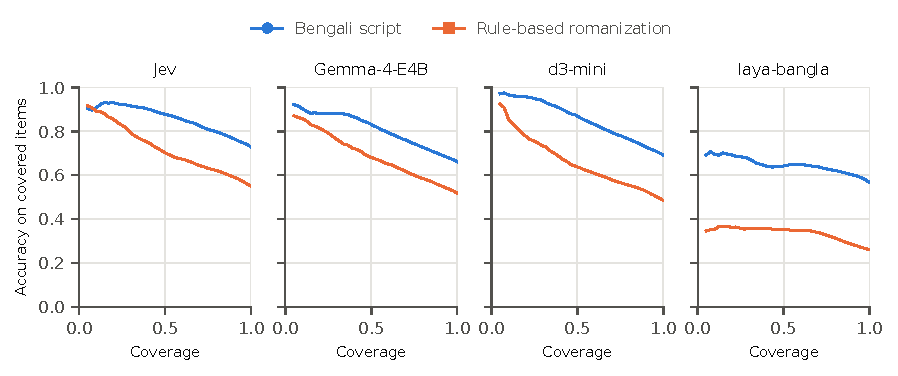
\includegraphics[width=\linewidth]{figures/fig4_risk_coverage}
\caption{Accuracy on the covered items as coverage grows from the most confident answers.}
\label{fig:rc}
\end{figure}

A confidence gate set on Bengali development text to reach \gateTarget\% accuracy does not carry over.
On MASSIVE, Jev accepts \gatejevNatCov\% of Bengali items (\gatejevNatN{} items) at \gatejevNatAcc\% accuracy, but only \gatejevRomCov\% of rule-based romanized items (\gatejevRomN{}), at \gatejevRomAcc\%. d3-mini accepts \gateminiNatCov\% (\gateminiNatN{}) at \gateminiNatAcc\% and \gateminiRomCov\% (\gateminiRomN{}) at \gateminiRomAcc\%.
For laya-bangla the accepted rule-based romanized items are \gatelayabnRomAcc\% accurate, but only \gatelayabnRomN{} items are accepted, so that figure is close to anecdote.
So for Jev and d3-mini the gate keeps its accuracy by refusing most rule-based romanized input, and for laya-bangla it fails.
This rests on one task and, for some models, on few accepted items, so I treat it as exploratory.

\subsection{Option-order sensitivity}
Across three rotations of the options, Jev gives the same answer \consjev\% of the time, d3-nano \consnano\%, d3-lite \conslite\% and Gemma-4-E4B \consgemma\%.
The encoders are far less stable: laya-bangla \conslayabn\%, Laya-multilingual \conslayaml\%, Julia-1 \consjulia\% (Figure~\ref{fig:rot}; per task in Table~\ref{tab:rot}).
\begin{figure}[t]
\centering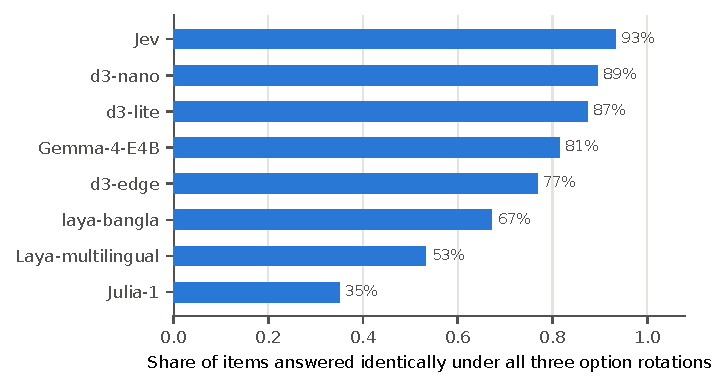
\includegraphics[width=.7\linewidth]{figures/fig5_rotation}
\caption{Share of items answered identically under all three option rotations, over all tasks.}
\label{fig:rot}
\end{figure}

\subsection{Checks on the harness}
\label{sec:audit}
Before trusting any of this I tried to reproduce other people's numbers.
From the Jev authors' released responses, Belebele ben\_Beng accuracy is \jevBelebeleZenodo; my own run gives \jevBelebele.
For Laya-multilingual I get MASSIVE \layamlNativeMassive{} and SIB-200 \layamlNativeSib, against 0.18 and 0.57 to 0.58 reported by the laya-bangla authors. For laya-bangla I get SIB-200 \layabnNativeSib{} against their 0.76.
Resending 300 Jev requests gave the same answer \jevRetestSame\% of the time, and a newer Laya package version changed no answer on 6{,}563 requests.
One comparison I could not make: laya-bangla's authors report MASSIVE 0.81 with a two-step scenario-then-intent protocol, and I ask one 60-way question and get \acclayabnMasNat.
The study used \jevRequests{} Jev requests, about \jevTokensM{}M input tokens and \$\jevUsd{} at \$0.042 per million, plus about \gpuHours{} GPU hours on Kaggle.
I measured latency under mixed conditions, so it is not comparable across models, and I do not report it.

\section{Discussion}
\paragraph{What rule-based romanization can and cannot tell you.}
Rule-based romanization ranked the systems in nearly the same order as native-speaker romanization, and moved their answers further. For Jev, the rule-based text cost \dropjev{} points of accuracy on average over four tasks, and the same system kept its answer on \dakjevRule{} of the Dakshina sentences under rule-based romanization against \dakjevNs{} under native-speaker romanization.
So a penalty measured on tool-made text is an upper bound on what a system loses on text people write, for the systems and sentences I tested, and not a good estimate of it.
I do not know why the native speakers' spelling is easier. A plausible reason is that people spell common words, and English loan words, the way models have seen them in web text; I did not test that.

\paragraph{Choosing a model.}
On Bengali script d3-mini, d3-nano and Gemma-4-E4B come within a few points of Jev on several tasks, so the hosted model's advantage here is modest.
Gemma-4-E4B is the most robust open model to rule-based romanization, and also among the worst calibrated before scaling (ECE \ecegemmaNatRaw), which temperature scaling mostly removes.
The encoders need care. Their answers change with option order, and Laya-multilingual's SentNoB score moved by more than ten points with the wording of the question.

\section{Limitations}
The Dakshina comparison measures agreement with a system's own Bengali answer, not accuracy, because the sentences have no labels; a system that is wrong on the Bengali sentence can still agree with itself. It uses Wikipedia sentences and a single seven-way topic question, so it does not show that the same gap holds on the five tasks.
The sentences were romanized by native speakers, but I do not know how many, or how representative they are of everyday typing on phones and social media.
The five tasks use rule-based romanization only. XNLI-bn and MASSIVE are translations, so SentNoB is the only native Bengali text.
d3-flash ran 4-bit on subsets, Kev ran only on the test sets and on Dakshina, the larger Kev and d3 models were not run, and Julia-1 cannot take MASSIVE.
Contamination is unknown for Jev, Gemma and the Qwen-based d3 models, and laya-bangla was trained on MASSIVE and SIB-200 training splits.
The SentNoB split I used is a third-party mirror whose provenance I could not verify.
I use one prompt format per model family, and Laya's wording sensitivity shows that this can move a result.
The calibration and gate results are exploratory and use no multiplicity correction.

\section{Conclusion}
On five Bengali tasks Jev leads, several small open models come close on Bengali script, and the open models' overconfidence is largely fixed by one temperature on Bengali text but less fully on rule-based romanized text.
Rule-based romanization lowers every system's accuracy, but it overstates the effect of real typing: on Bengali sentences that native speakers romanized, all twelve systems kept their Bengali-script answer more often than under the rule-based text, while ranking in nearly the same order.
Measuring the effect on labelled tasks needs Banglish typed by many writers for sentences that have labels.

\paragraph{Availability.}
The repository is at \url{https://github.com/ihpolash/system-one-testing-for-bengali}. It holds the harness, the analysis code that generates every table and number in this paper, the summary result tables, item-level predictions for the open models and per-sentence answers for the Dakshina experiment, SHA-256 checksums for the released files, the exact model identifiers and settings (\texttt{docs/MODELS.md}) and the question structure for each task (\texttt{docs/PROMPTS.md}). The test-set predictions contain no dataset text except Belebele's option labels, which are the Bengali option texts (CC BY-SA 4.0). The Dakshina predictions are keyed by sentence identifier; \texttt{data/make\_dakshina.py} rebuilds the sentences from the public dataset (CC BY-SA 4.0). SentNoB is distributed under a no-derivatives licence, so the repository does not contain its text. Jev's raw responses and probability vectors are not included (provider terms); only its top choice and confidence are released for the Dakshina sentences.

\section*{Declaration on the use of generative AI}
The author used an AI assistant (Claude, Anthropic) for implementation support, analysis and figure scripting, and for drafting and editing this manuscript. All of that work was carried out under the author's direction and review. No generative AI was used to produce any evaluation text: the Latin-script text comes from the Dakshina dataset and from rule-based and corpus-based romanizers. The research questions, benchmark design, evaluation protocol and the interpretation of the results are the author's. All numerical results in the tables and text are generated by the released analysis code from the stored results, and every reference was verified by the author against its primary source. The author takes full responsibility for all content of this paper, irrespective of how it was drafted.

\bibliographystyle{plainnat}
\bibliography{refs}

\appendix
\section{Additional tables}
\begin{table}[h]
\centering\footnotesize
\resizebox{\linewidth}{!}{\begin{tabular}{@{}lccccc@{}}\toprule
Model & Belebele & SIB-200 & XNLI-bn & MASSIVE & SentNoB \\\midrule
Jev & 0.918 [0.897, 0.936] & 0.897 [0.853, 0.936] & 0.751 [0.729, 0.772] & 0.757 [0.735, 0.779] & 0.623 [0.596, 0.647] \\
Gemma-4-E4B & 0.773 [0.743, 0.801] & 0.853 [0.804, 0.897] & 0.631 [0.606, 0.655] & 0.689 [0.667, 0.713] & 0.590 [0.566, 0.615] \\
d3-mini & 0.727 [0.697, 0.758] & 0.838 [0.789, 0.887] & 0.729 [0.705, 0.752] & 0.749 [0.728, 0.771] & 0.579 [0.555, 0.604] \\
d3-nano & 0.702 [0.671, 0.733] & 0.848 [0.799, 0.897] & 0.746 [0.725, 0.768] & 0.705 [0.681, 0.730] & 0.592 [0.568, 0.614] \\
Kev-4B & 0.561 [0.528, 0.592] & 0.779 [0.721, 0.833] & 0.624 [0.603, 0.648] & 0.575 [0.551, 0.600] & 0.536 [0.511, 0.556] \\
d3-lite & 0.577 [0.542, 0.609] & 0.760 [0.701, 0.819] & 0.704 [0.681, 0.726] & 0.624 [0.600, 0.647] & 0.535 [0.511, 0.558] \\
laya-bangla & 0.313 [0.283, 0.344] & 0.750 [0.686, 0.814] & 0.625 [0.599, 0.650] & 0.575 [0.547, 0.602] & 0.464 [0.437, 0.488] \\
d3-edge & 0.409 [0.377, 0.441] & 0.475 [0.407, 0.544] & 0.523 [0.497, 0.548] & 0.243 [0.223, 0.264] & 0.472 [0.451, 0.498] \\
Kev-0.8B & 0.374 [0.341, 0.407] & 0.632 [0.564, 0.701] & 0.469 [0.445, 0.491] & 0.372 [0.347, 0.397] & 0.359 [0.337, 0.380] \\
Laya-multilingual & 0.287 [0.259, 0.314] & 0.588 [0.515, 0.657] & 0.635 [0.612, 0.660] & 0.179 [0.161, 0.199] & 0.263 [0.244, 0.283] \\
Julia-1 & 0.287 [0.258, 0.316] & 0.520 [0.456, 0.588] & 0.382 [0.359, 0.406] & -- & 0.403 [0.379, 0.424] \\
\bottomrule\end{tabular}
}
\caption{Accuracy on Bengali script with 95\% cluster-bootstrap intervals (SentNoB: macro-F1).}
\label{tab:ci}
\end{table}
\begin{table}[h]
\centering\footnotesize
\begin{tabular}{@{}lccccc@{}}\toprule
Model & Belebele & SIB-200 & XNLI-bn & MASSIVE & SentNoB \\\midrule
Jev & 0.9 / 93\% & 1.0 / 97\% & 0.5 / 97\% & 1.7 / 89\% & 0.9 / 95\% \\
Gemma-4-E4B & 1.4 / 74\% & 0.5 / 93\% & 3.3 / 86\% & 4.3 / 70\% & 0.1 / 94\% \\
d3-nano & 1.1 / 82\% & 0.5 / 96\% & 0.7 / 96\% & 1.1 / 85\% & 0.4 / 95\% \\
d3-lite & 1.2 / 82\% & 1.0 / 96\% & 0.7 / 96\% & 0.5 / 80\% & 1.2 / 92\% \\
laya-bangla & 2.1 / 28\% & 2.0 / 94\% & 1.2 / 89\% & 0.3 / 66\% & 2.8 / 88\% \\
d3-edge & 0.3 / 75\% & 4.4 / 83\% & 1.9 / 92\% & 3.3 / 49\% & 1.4 / 90\% \\
Laya-multilingual & 1.1 / 15\% & 1.0 / 84\% & 0.1 / 91\% & 8.7 / 29\% & 4.6 / 80\% \\
Julia-1 & 1.8 / 31\% & 2.9 / 74\% & 1.9 / 24\% & -- & 10.8 / 45\% \\
\bottomrule\end{tabular}

\caption{Spread of accuracy across the three option rotations (points) / share of items answered identically under all three.}
\label{tab:rot}
\end{table}
\begin{table}[h]
\centering\footnotesize
\begin{tabular}{@{}lcccccc@{}}\toprule
 & \multicolumn{2}{c}{XNLI-bn} & \multicolumn{2}{c}{MASSIVE} & \multicolumn{2}{c}{SentNoB} \\\cmidrule(lr){2-3}\cmidrule(lr){4-5}\cmidrule(l){6-7}
Model & Bengali & Rule & Bengali & Rule & Bengali & Rule \\\midrule
Jev & 0.088 & 0.197 & 0.087 & 0.081 & 0.202 & 0.161 \\
Gemma-4-E4B & 0.327 & 0.402 & 0.249 & 0.397 & 0.333 & 0.374 \\
d3-mini & 0.049 & 0.038 & 0.054 & 0.104 & 0.120 & 0.094 \\
d3-nano & 0.069 & 0.071 & 0.073 & 0.129 & 0.107 & 0.165 \\
Kev-4B & 0.238 & 0.316 & 0.270 & 0.101 & 0.170 & 0.205 \\
d3-lite & 0.059 & 0.057 & 0.048 & 0.272 & 0.120 & 0.187 \\
laya-bangla & 0.203 & 0.286 & 0.071 & 0.138 & 0.339 & 0.568 \\
d3-edge & 0.178 & 0.066 & 0.223 & 0.423 & 0.120 & 0.117 \\
Kev-0.8B & 0.173 & 0.131 & 0.166 & 0.053 & 0.192 & 0.247 \\
Laya-multilingual & 0.276 & 0.469 & 0.236 & 0.468 & 0.530 & 0.654 \\
Julia-1 & 0.420 & 0.532 & -- & -- & 0.444 & 0.456 \\
\bottomrule\end{tabular}

\caption{ECE (15 bins, no temperature scaling) within each task on the full test sets, for Bengali script and rule-based romanization. The mean of these per-task values over the three tasks is the primary ECE of Table~\ref{tab:cal}. d3-flash is omitted (subset).}
\label{tab:caltasks}
\end{table}
\begin{table}[h]
\centering\footnotesize
\begin{tabular}{@{}lcccc@{}}\toprule
 & \multicolumn{2}{c}{Brier score} & \multicolumn{2}{c}{Confidence $-$ accuracy} \\\cmidrule(lr){2-3}\cmidrule(l){4-5}
Model & Bengali & Rule-based & Bengali & Rule-based \\\midrule
Jev & 0.418 & 0.617 & +0.122 & +0.144 \\
Gemma-4-E4B & 0.637 & 0.849 & +0.303 & +0.391 \\
d3-mini & 0.432 & 0.649 & +0.069 & +0.073 \\
d3-nano & 0.429 & 0.731 & +0.081 & +0.121 \\
Kev-4B & 0.616 & 0.802 & +0.045 & +0.141 \\
d3-lite & 0.508 & 0.806 & +0.073 & +0.166 \\
laya-bangla & 0.650 & 0.983 & +0.159 & +0.331 \\
d3-edge & 0.744 & 0.852 & +0.173 & +0.201 \\
Kev-0.8B & 0.734 & 0.817 & +0.066 & +0.136 \\
Laya-multilingual & 0.909 & 1.216 & +0.347 & +0.530 \\
Julia-1 & 0.972 & 1.080 & +0.431 & +0.494 \\
\bottomrule\end{tabular}

\caption{Brier score and confidence minus accuracy on Bengali script and rule-based romanization (test sets, mean over XNLI-bn, MASSIVE and SentNoB, no temperature scaling). Positive values mean overconfident.}
\label{tab:calbrier}
\end{table}
\begin{table}[h]
\centering\footnotesize
\begin{tabular}{@{}lcccccc@{}}\toprule
 & \multicolumn{3}{c}{Probability shift (TV)} & \multicolumn{3}{c}{Mean top-option confidence} \\\cmidrule(lr){2-4}\cmidrule(l){5-7}
Model & Native-speaker & Natural-style & Rule-based & Native-speaker & Rule-based & Bengali \\\midrule
Jev & 0.262 & 0.336 & 0.324 & 0.749 & 0.711 & 0.848 \\
d3-flash (4-bit)$^\dagger$ & 0.324 & 0.399 & 0.392 & 0.632 & 0.597 & 0.764 \\
Gemma-4-E4B & 0.271 & 0.322 & 0.325 & 0.910 & 0.905 & 0.937 \\
d3-mini & 0.346 & 0.430 & 0.439 & 0.655 & 0.594 & 0.792 \\
d3-nano & 0.412 & 0.492 & 0.506 & 0.621 & 0.566 & 0.773 \\
Kev-4B & 0.310 & 0.382 & 0.383 & 0.550 & 0.498 & 0.655 \\
d3-lite & 0.453 & 0.506 & 0.529 & 0.570 & 0.511 & 0.759 \\
laya-bangla & 0.566 & 0.626 & 0.646 & 0.589 & 0.543 & 0.759 \\
d3-edge & 0.452 & 0.491 & 0.509 & 0.545 & 0.452 & 0.636 \\
Kev-0.8B & 0.412 & 0.465 & 0.480 & 0.515 & 0.466 & 0.605 \\
Laya-multilingual & 0.608 & 0.648 & 0.670 & 0.850 & 0.837 & 0.855 \\
Julia-1 & 0.528 & 0.547 & 0.565 & 0.806 & 0.850 & 0.830 \\
\bottomrule\end{tabular}

\caption{Dakshina sentences: mean total-variation distance between the probability vector on the Bengali sentence and on each romanization (0 is identical, 1 disjoint), and mean top-option confidence on each spelling. d3-flash is 4-bit and covers a 500-sentence subset.}
\label{tab:daktv}
\end{table}
\end{document}
